\section{Introducción y generalidades (2023-08-17)}
\begin{frame}\frametitle{Contexto y definiciones}
  \begin{itemize}
  \item La palabra \textit{robot} tiene su origen en la obra \textit{Rossum's Universal Robots} del escritor checo $Karel \,\check{C}apeck$, publicada en 1921, y su significado es ``trabajo duro''.
  \item Latombe (1991) define un robot como un dispositivo mecánico versátil equipado con sensores y actuadores bajo el control de un sistema de cómputo \cite{Latombe1991MotionPlanning}.
  \item Arkin (1998) propone que un robot inteligente es una máquina capaz de extraer información de su ambiente y usar el conocimiento acerca de su mundo para moverse de manera segura y significativa, con un propósito específico \cite{Arkin1998BehBasedRobo}.
  \item Robótica es la ciencia que estudia la conexión inteligente entre la percepción y la acción. 
  \end{itemize}
\end{frame}

\begin{frame}\frametitle{Áreas de la Robótica}
  
  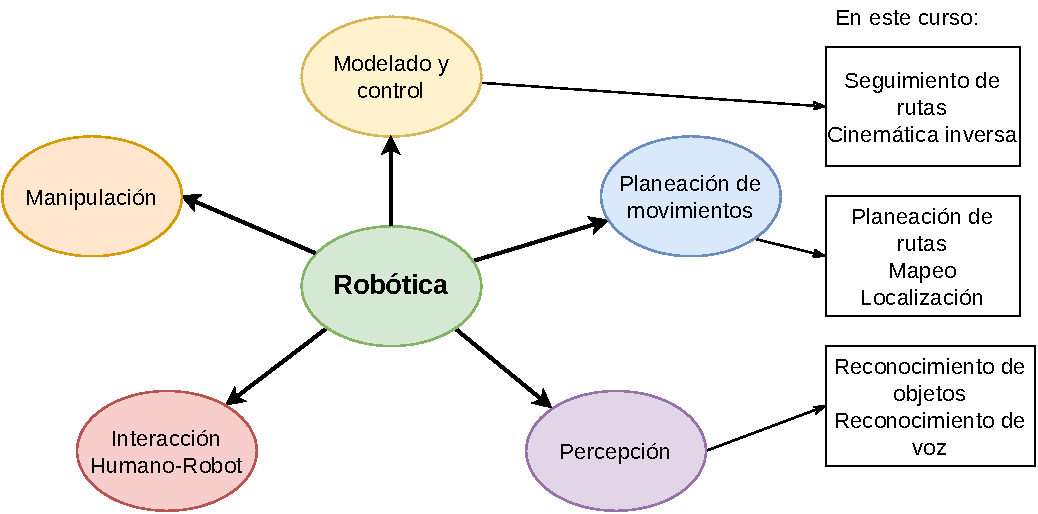
\includegraphics[width=0.9\textwidth]{Figures/RoboticsAreas.pdf}
\end{frame}

\begin{frame}\frametitle{Componentes de un robot}
  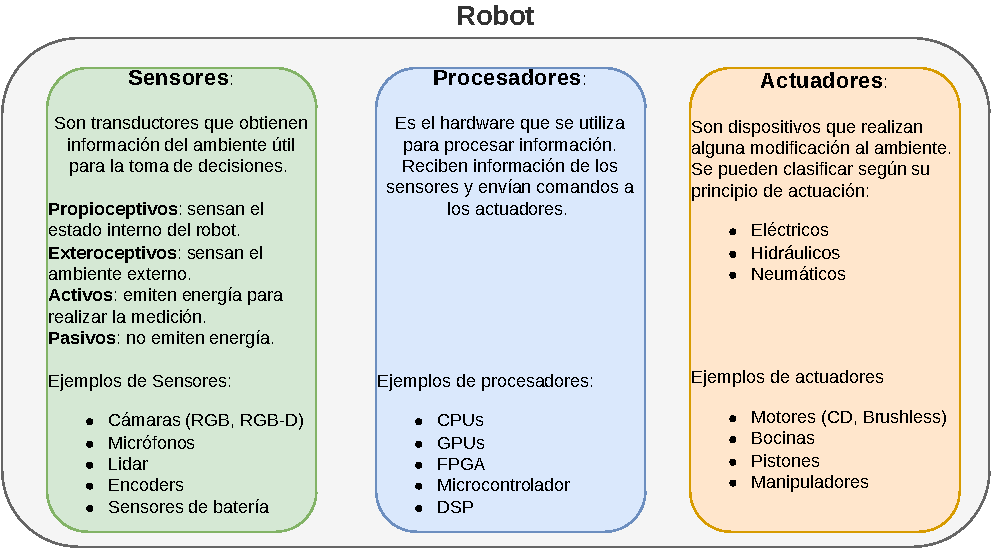
\includegraphics[width=0.9\textwidth]{Figures/RobotComponents.pdf}
\end{frame}

\begin{frame}\frametitle{Conceptos Básicos}
  \begin{itemize}
  \item \textbf{Configuración:} es la descripción de la posición en el espacio de todos los puntos del robot. Se denota con $q$.
  \item \textbf{Espacio de configuraciones:} es el conjunto $Q$ de todas las posibles configuraciones. 
  \item \textbf{Grados de libertad:} número mínimo de variables independientes para describir una configuración. En este curso, la base móvil del robot tiene 3 GdL, la cabeza tiene 2 GDL y cada brazo tiene 7 GDL más 1 GdL para el gripper. En total, el robot tiene 21 GdL. 
  \end{itemize}
  \textbf{Propiedades del robot:}
  \begin{itemize}
  \item \textbf{Holonómico:} el robot puede moverse instantáneamente en cualquier dirección del espacion de configuraciones. Comunmente se logra mediante ruedas de tipo \textit{Mecanum} u \textit{Omnidireccionales}. 
  \item \textbf{No holonómico:} existen restricciones de movimiento en velocidad pero no en posición. Son restricciones que solo se pueden expresar en términos de la velocidad pero no pueden integrarse para obtener una restricción en términos de posición. Ejemplo: un coche sólo puede moverse en la dirección que apuntan las llantas delanteras, sin embargo, a través de maniobras puede alcanzar cualquier posición y orientación. El robot de este curso es no holonómico. 
  \end{itemize}
\end{frame}

\begin{frame}\frametitle{Conceptos Básicos}
  \textbf{Propiedades de los algoritmos:}
  \begin{itemize}
  \item \textbf{Complejidad:} cuánta memoria y cuánto tiempo se requiere para ejecutar un algoritmo, en función del número de datos de entrada (número de grados libertad, número de lecturas de un sensor, entre otros).
  \item \textbf{Optimalidad:} un algoritmo es óptimo cuándo encuentra una solución que minimiza una función de costo.
  \item \textbf{Completitud:} un algoritmo es completo cuando garantiza encontrar la solución siempre que ésta exista. Si la solución no exite, indica falla en tiempo finito.
    \begin{itemize}
    \item Completitud de resolución: la solución existe cuando se tiene una discretización. 
    \item Completitud probabilística: la probabilidad de encontrar la solución tiende a 1.0 cuando el tiempo tiende a infinito.
    \end{itemize}
  \end{itemize}
  Una explicación más detallada se puede encontrar en el Cap. 3 de \cite{choset2005principles}.
\end{frame}

